\chapter{Stringology}

\begin{tcolorbox}[colframe=black!3!white]
  \textbf{Inhalt dieses Kapitels}:
  \tcblower{} 
  \begin{itemize}
    \item Strings sortieren
    \item Patterns suchen
    \item Datenkompression
  \end{itemize}
\end{tcolorbox}

\section{Strings sortieren}\label{sec:stringSorting}

Naive Sortierverfahren, wie sie aus der Vorlesung ``Algorithmen 1'' bekannt sind, sind beim Sortieren von Strings ineffizient, deswegen gibt es für das Sortieren von Strings andere Algorithmen. Ein solcher ist der \term{Multikey Quicksort}\label{def:multikeyQuicksort}\index{Multikey Quicksort}-Algorithmus:

\begin{figure}[H]
  \begin{pseudocode}
    \textbf{\textsc{mkqSort}} (\( S \): String Seq, \( l : \N \)): String Seq \\
    \textbf{assert} \( \forall e, e' \in S : e[1\dots l-1] = e'[1\dots l-1] \) \\
    \textbf{if} \( \left\vert S \right\vert \leq 1 \) \textbf{then return} \( S \) \\
    pick \( p \in S \) randomly \\
    \textbf{return} concatenation of \\
    \phantom{\enskip} \textsc{mkqSort} (\( \langle e \in S : e[l] < p[l] \rangle, l \)), \\
    \phantom{\enskip} \textsc{mkqSort} (\( \langle e \in S : e[l] = p[l] \rangle, l+1 \)), \\
    \phantom{\enskip} \textsc{mkqSort} (\( \langle e \in S : e[l] > p[l] \rangle, l \))
  \end{pseudocode}
  \caption{Pseudocode-Implementierung des Multikey-Quicksort-Algorithmus}
\end{figure}

Dieser Algorithmus sortiert eine String-Sequenz und nimmt an, dass die ersten \( l-1 \) Buchstaben bereits sortiert wurden. \\
Zuerst wird ein zufälliges Pivotelement gewählt. Danach wird die übergebene Sequenz an Strings wird in drei Teilsequenzen geteilt:
\begin{enumerate}
  \item Sequenz an Strings, deren \( l \)-ter Buchstabe kleiner ist als der \( l \)-te Buchstabe des Pivotelements.
  \item Sequenz an Strings, deren \( l \)-ter Buchstabe derselbe ist wie der \( l \)-te Buchstabe des Pivotelements.
  \item Sequenz an Strings, deren \( l \)-ter Buchstabe größer ist als der \( l \)-te Buchstabe des Pivotelements.
\end{enumerate}
Auf die erste und dritte Teilsequenz wird der Algorithmus nun rekursiv mit dem selben Parameter \( l \) ausgeführt, da die Buchstaben an der \( l \)-ten Position nicht übereinstimmen (müssen) --- auf die zweite Teilsequenz wird der Algorithmus rekursiv mit dem Parameter \( l+1 \) ausgeführt, weil hier die \( l \)-ten Buchstaben aller Wörter in der Sequenz gleich sind. \\
Die Laufzeit des Algorithmus ist in \( O(\left\vert S \right\vert \log \left\vert S \right\vert + d) \), wobei \( d \) die Summe der eindeutigen Präfixe der Strings in \( S \) ist.

\section{Pattern Matching}\label{sec:patternMatching}

\emph{Hinweis}: In diesem Abschnitt sind Arrays \( 1 \)-basiert. \\

In diesem Abschnitt wird es darum gehen, alle oder zumindest ein Vorkommen eines \term{Patterns}\index{Pattern} \( P = p_1\dots p_m \) in einem gegebenen \term{Text}\index{Text} \( T = t_1\dots t_n \) zu finden. Im Allgemeinen ist \( n \gg m \), also der Text wesentlich länger als das Pattern, das wir in ihm suchen. 

\subsection{Naives Pattern Matching}
Das naive Vorgehen ist, an jeder Position von \( T \) zu schauen, ob an dieser das gesuchte Pattern vorkommt. Offensichtlich ist dieser Algorithmus in \( O(nm) \), da im schlimmsten Fall für jede Position des Textes das gesamte Pattern durchlaufen werden muss. Dieser Algorithmus kann folgendermaßen implementiert werden:
\begin{figure}[H]
  \begin{pseudocode}
    \textbf{\textsc{naivePatternMatch}} (\( P \), \( T \)) \\
    \( i \),\( j \coloneqq 1 \) \\
    \textbf{while} \( i \leq n-m+1 \) \\
    \phantom{\enskip} \textbf{while \( j \leq m \wedge t_{i+j-1} = p_j \)} \textbf{do} \( j \)++ \\
    \phantom{\enskip} \textbf{if \( j > m \)} \textbf{then return} ``\( P \) occurs at pos \( i \) in \( T \)'' \\
    \phantom{\enskip} \( i \)++ \\
    \phantom{\enskip} \( j \coloneqq 1 \)
  \end{pseudocode}
  \caption{Pseudocode-Implementierung des naiven Pattern-Matching-Algorithmus}
\end{figure}

\subsection{Knuth-Morris-Pratt}
Ein anderer Algorithmus zum Finden von Patterns in einem gegebenen Text ist der \term{Knuth-Morris-Pratt-Algorithmus}\label{def:kmpAlgorithmus}\index{Knuth-Morris-Pratt-Algorithmus}. Dieser hat sogar optimale Laufzeit, nämlich \( O(n+m) \). \\
Idee dieses Algorithmus ist es, das Pattern eleganter nach vorne zu verschieben, wenn es einen Mismatch zwischen Text und Pattern gibt. Hierfür brauchen wir ein Hilfswerkzeug: \\
Für einen String \( S \) mit Länge \( k \) sei \( \alpha(S) \) die Länge des Längsten Präfixes von \( S_{1\dots k-1} \), das auch Suffix von \( S_{2\dots k} \) ist.\footnote{Wir lassen absichtlich bei Betrachtung des Präfixes den letzten und bei Betrachtung des Suffixes den ersten Buchstaben weg, damit \( \alpha(S) = 0 \) ist, wenn \( \left\vert S \right\vert = k = 1 \) ist.} 

\begin{figure}[H]
  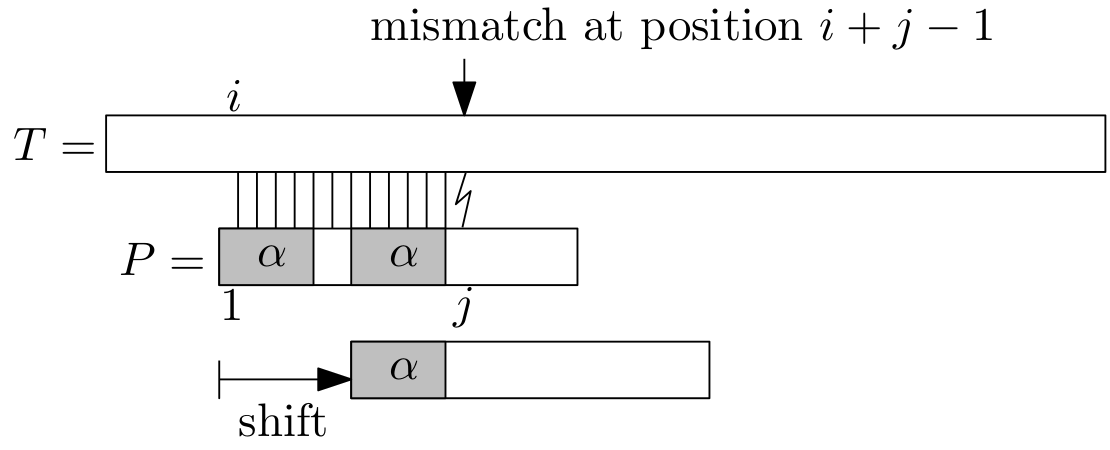
\includegraphics[width=.5\textwidth]{KMP}
  \captionsetup{width=.5\textwidth}
  \caption{Idee beim Verschieben des Patterns: \( \alpha \) wurde bereits gematcht. Früher als mit dem bereits gematchten Suffix kann das nächste Vorkommen von \( P \) nicht auftauchen, also kann mann \( P \) direkt um \( j - 1 - \alpha \) verschieben}
\end{figure}

Der Algorithmus besteht aus zwei Teilen:
\begin{enumerate}
  \item \textbf{Border-Array berechnen} (\( O(m) \)). Damit die oben erläuterten Verschiebungen nachher effizient durchgeführt werden können, berechnen wir für das leere Wort \emph{und} jeden Buchstaben in \( P \) einen \( \alpha \)-Wert. Diese Werte ergeben das \term{Border-Array}\label{def:borderArray}\index{Border-Array}:

  \begin{minipage}{.55\textwidth}
    \begin{equation*}
      \text{border}[j] = \begin{cases}
        -1\text{,} &\text{falls } j = 1 \\
        \alpha(P_{1 \dots j-1})\text{,} &\text{sonst}
      \end{cases}\text{.}
    \end{equation*}
  \end{minipage}
  \hfill
  \begin{minipage}{.35\textwidth}
    \begin{figure}[H]
      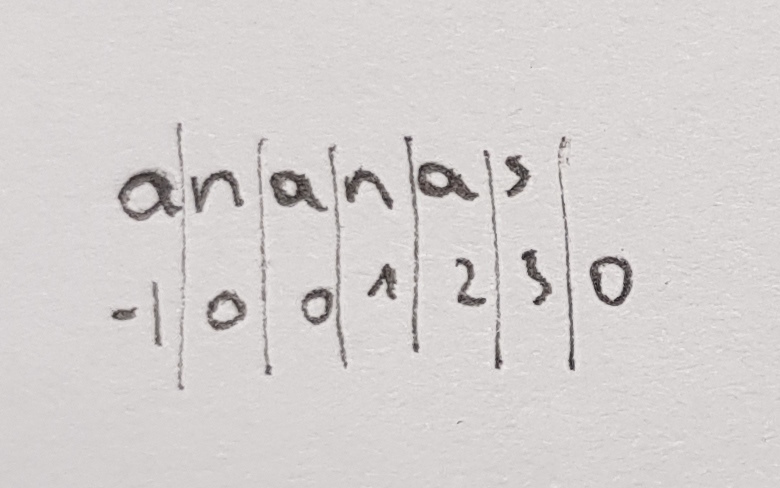
\includegraphics[width=.8\textwidth]{borderArray}
      \caption{Beispiel für das Border-Array eines Patterns}
    \end{figure}
  \end{minipage} \\

  \item \textbf{Pattern matchen} (\( O(n) \)). Nun verwenden wir das erstellte Border-Array, um Vorkommnisse von \( P \) in \( T \) zu finden. Wir starten sowohl im Text als auch im Pattern an Position 1 und fangen an zu matchen. Kommt es an Position \( 1 \leq j \leq m \) des Patterns zu einem Mismatch, so können wir \( P \) direkt um \( j - \text{border}[j] - 1 \) verschieben. In Pseudocode sieht das so aus:
  \begin{pseudocode}
    \textbf{\textsc{KMPMatch}} (P,T) \\
    \( i,j \coloneqq 1 \) \\
    \textbf{while} \( i \leq n - m + 1 \) \\
    \phantom{\enskip} \textbf{while} \( j \leq m \wedge t_{i+j-1} = p_j \) \textbf{do} \( j \)++ \\
    \phantom{\enskip} \textbf{if} \( j > m \) \textbf{then return} ``\( P \) occurs at pos \( i \) in \( T \) '' \\
    \phantom{\enskip} \( i \) += \( j - \text{border}[j] + 1 \) \\
    \phantom{\enskip} \( j \coloneqq \max\left \{ 1, \text{border}[j]+1 \right \} \)
  \end{pseudocode}
\end{enumerate}

Eine Ausführung des Algorithmus kann also folgendermaßen aussehen:
\begin{figure}[H]
  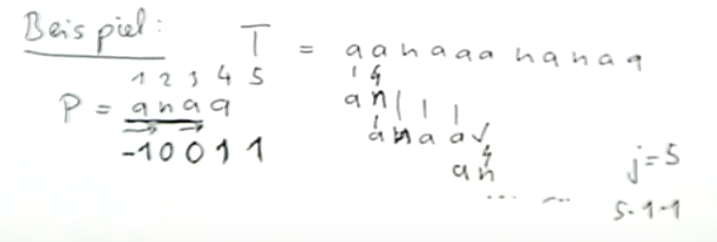
\includegraphics[width=.6\textwidth]{kmpBeispiel}
  \caption{Beispiel für das Verwenden des Knuth-Morris-Pratt-Algorithmus}
\end{figure}

\subsection{Suffix-Arrays}

Im Folgenden werden Arrays wieder mit Position \( 0 \) beginnen. Wir verwenden desweiteren folgende Festlegungen:
\begin{itemize}
  \item Ein \term{String}\index{String} ist ein Array von Buchstaben,
  \begin{equation*}
    S[0\dots n) \coloneqq S[0\dots n-1] \coloneqq [S[0],\dots,S[n-1]]\text{.}
  \end{equation*}
  \item Das \term{Suffix}\index{Suffix} \( S_i \) sei der Substring \( S[i\dots n) \) von \( S \).
  \item Wir setzen an das Ende jedes Strings ausreichend viele \term{Endmarkierungen}\index{Endmarkierung}: \( S[n] \coloneqq S[n+1] \coloneqq \cdots \coloneqq 0 \). \( 0 \) sei per Definition kleiner als alle anderen vorkommenden Zeichen.
\end{itemize}

Das \term{Suffix-Array}\index{Suffix-Array} eines Strings lässt sich nun folgendermaßen konstruieren:

\begin{minipage}{.65\textwidth}
  \begin{enumerate}
    \item Bilde die Menge aller Suffixe \( S_i \) (\( i = 0,\dots,n-1 \)) des Strings.
    \item Sortiere die Menge aller Suffixe des Strings (z.B. mit \hyperref[def:multikeyQuicksort]{Multikey Quicksort}).
  \end{enumerate}
\end{minipage}
\hfill
\begin{minipage}{.35\textwidth}
  \begin{figure}[H]
    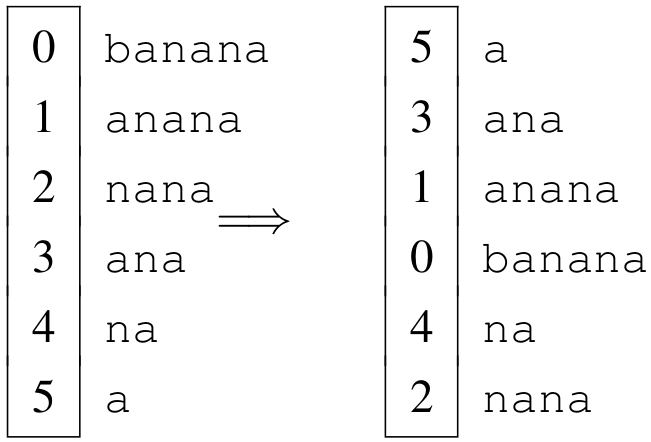
\includegraphics[width=.8\textwidth]{suffixArray}
    \caption{Beispiel für die Konstruktion des Suffix-Arrays des Strings ``\emph{banana}''}
  \end{figure}
\end{minipage}

Mithilfe dieses Suffix-Arrays lassen sich später viele Suchprobleme in Linearzeit lösen. Beispielsweise ist die Suche nach dem längsten Substring, der (eventuell mit Überschneidung) zweimal im Text vorkommt, linear --- dafür muss nach Berechnung des Suffix-Arrays der längste String gefunden werden, der Präfix von zwei Strings im Suffix-Array ist (im Beispiel oben wäre das ``\emph{ana}'').

\subsection{Berechnung des Suffix-Arrays in Linearzeit}\label{sec:SALinear}

Das Suffix-Array eines Strings lässt sich in Linearzeit berechnen.\footnote{Kärkkäinen, Sanders, Burkhardt: Linear Work Suffix Array Construction} Hier soll lediglich das Prinzip erläutert werden, genauere Angaben gibt es im Paper.

Wir betrachten den String
\begin{equation*}
  T[0,n) = \ \underset{\texttt{0}}{\texttt{x}}\ \underset{\texttt{1}}{\texttt{a}}\ \underset{\texttt{2}}{\texttt{b}}\ \underset{\texttt{3}}{\texttt{b}}\ \underset{\texttt{4}}{\texttt{a}}\ \underset{\texttt{5}}{\texttt{d}}\ \underset{\texttt{6}}{\texttt{a}}\ \underset{\texttt{7}}{\texttt{b}}\ \underset{\texttt{8}}{\texttt{b}}\ \underset{\texttt{9}}{\texttt{a}}\ \underset{\texttt{10}}{\texttt{d}}\ \underset{\texttt{11}}{\texttt{o}}\text{.}
\end{equation*}
Unser Ziel ist das Suffix-Array
\begin{equation*}
  \text{SA} = \left( 12,1,6,4,9,3,8,2,7,5,10,11,0 \right)\text{.}
\end{equation*}

Wir gehen wie folgt vor:
\begin{enumerate}
  \setcounter{enumi}{-1}
  \item \textbf{Suffixe wählen}. \quad Sei 
  \begin{equation*}
    B_k = \left \{ i \in [0,n] \ : \ i \mod 3 = k \right \}
  \end{equation*}
  und \( C = B_1 \cup B_2 \) sowie \( S_C \) die Menge der entsprechenden Suffixe. \( C \) ist also die Menge aller Positionen in \( T \), an denen Suffixe mit einer nicht durch \( 3 \) teilbaren Länge beginnen. Hier ist \( C = \left \{ 1,4,7,10,2,5,8,11 \right \} \).
  
  \item \textbf{Gewählte Suffixe sortieren}. \quad Wir fügen am Ende von \( T \) beliebig viele \texttt{0} hinzu und bilden zuerst für \( k = 1,2 \) die Strings
  \begin{equation*}
    R_k = [t_k t_{k+1} t_{k+2}][t_{k+3}t_{k+4}t_{k+5}]\cdots[t_{\max B_k}t_{\max B_{k}+1}t_{\max B_k +2}]\text{.}
  \end{equation*}
  Der Charaktere von \( R_k \) sind also Tripel. Das letzte Tripel ist immer eindeutig, weil \( t_{\max B_k + 2} = 0 \). Sei \( R = R_1 \odot R_2 \).

  Hier ist
  \begin{equation*}
    R = [\texttt{abb}][\texttt{ada}][\texttt{bba}][\texttt{do0}][\texttt{bba}][\texttt{dab}][\texttt{bad}][\texttt{o00}]\text{.}
  \end{equation*}

  Die Ordnung der Suffixe von \( R \) stimmt mit der Ordnung der Suffixe \( S_i \) überein, deswegen genügt es, die Suffixe von \( R \) zu sortieren.

  Wir sortieren \( R \) nun, indem wir die einzelnen Charaktere von \( R \) sortieren und durch ihren Rang in \( R \) ersetzen:
  \begin{equation*}
    \text{SA}_{R} = \left( 8,0,1,6,4,2,5,3,7 \right)\text{.}
  \end{equation*}

  Nun weisen wir jedem Suffix einen Rang zu. Dazu sei \( \text{rank}(S_i) \) der Rang von \( S_i \) in \( C \). Für \( i \in B_0 \) sei \( \text{rank}(S_i) \) nicht definiert.

  Hier ist \( \text{rank}(S_i) = \ \perp \ 1 \ 4 \ \perp \ 2 \ 6 \ \perp \ 5 \ 3 \ \perp \ 7 \ 8 \  \perp \ 0 \ 0 \).

  \item \textbf{Restliche Suffixe sortieren}. \quad Jeder Suffix \( S_i \in S_{B_0} \) sei dargestellt durch \( \left( t_i, \text{rank}(S_{i+1}) \right) \). Da wir alle anderen Suffixe oben schon sortiert haben ist \( \text{rank}(S_{i+1}) \) hier stets definiert.

  Offensichtlich ist
  \begin{equation*}
    S_i \leq S_j \Leftrightarrow \left( t_i, \text{rank}(S_{i+1}) \right) \leq \left( t_j, \text{rank}(S_{j+1}) \right)\text{,}
  \end{equation*}
  also lassen sich die Paare Radix-sortieren.

  Hier ist
  \begin{equation*}
    S_{12} < S_{6} < S_{9} < S_3 < S_0\text{,} \quad \text{weil} \quad \left( \texttt{0}, 0 \right) < \left( \texttt{a}, 5 \right) < \left( \texttt{a}, 7 \right) < \left( \texttt{b}, 2 \right) < \left( \texttt{x}, 1 \right)\text{.}
  \end{equation*}

  \item \textbf{Zusammenführen}. \quad Das Zusammenführen erfolgt vergleichsbasiert. Beim Vergleichen on \( S_i \in S_C \) mit \( S_j \in S_{B_0} \) unterscheiden wir zwei Fälle:
  \begin{align*}
    i \in B_1: \quad &S_i \leq S_j \Leftrightarrow \left( t_i, \text{rank}(S_{i+1}) \right) \leq \left( t_j, \text{rank}(S_{j+1}) \right) \\
    i \in B_2: \quad &S_i \leq S_j \Leftrightarrow \left( t_i, t_{i+1}, \text{rank}(S_{i+2}) \right) \leq \left( t_j, t_{j+1}, \text{rank}(S_{j+2}) \right)
  \end{align*}

  Hier ist z.B. \( S_1 < S_6 \) weil \( \left( \texttt{a}, 4 \right) < \left( \texttt{a}, 5 \right) \) und \( S_3 < S_8 \) weil \( \left( \texttt{b}, \texttt{a}, 6 \right) < \left( \texttt{b}, \texttt{a}, 7 \right) \).
\end{enumerate}

\subsection{Suchen in Suffix-Arrays}

Um ein Pattern in einem String zu finden, zu dem man das Suffix-Array konstruiert hat, muss man lediglich ein Suffix finden, dass das gesuchte Pattern als Präfix hat. Man kann so beispielsweise mit binärer Suche in \( O(m\log n) \) ein Vorkommen von \( P \) in \( T \) finden.

Nutzen wir eine zusätzliche Struktur, das \term{LCP-Array}\index{LCP-Array} --- dieses speichert in \( \text{LCP}[i] \) die Länge des längsten gemeinsamen Präfixes von \( \text{SA}[i] \) und \( \text{SA}[i-1] \) --- so können wir die Suchzeit auf \( O(m + \log n) \) reduzieren.

\begin{figure}[H]
  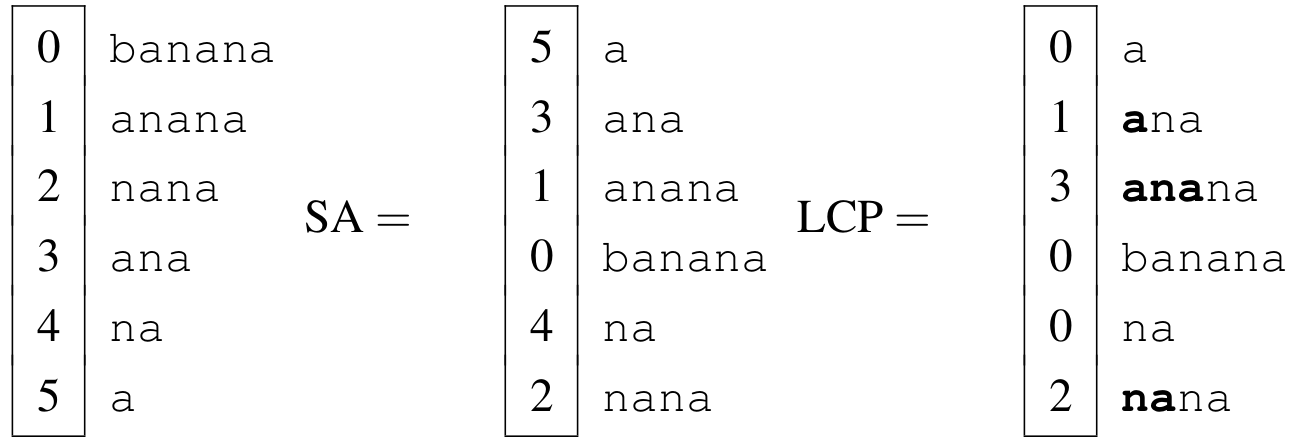
\includegraphics[width=0.6\textwidth]{LCPArray}
  \caption{Suffixe, Suffix-Array und LCP-Array des Strings ``\emph{banana}''}
\end{figure}

Um das LCP-Array berechnen zu können brauchen wir das \term{invertierte Suffix-Array}\index{Suffix-Array!invertiert}. Dieses gibt Aufschluss darüber, wo im Suffix-Array ein bestimmter Suffix steht. Offensichtlich ist \( \text{SA}^{-1}[\text{SA}[i]] = i \).

Der Algorithmus sieht folgendermaßen aus (\( O(n) \)):

\begin{pseudocode}
  \textbf{\textsc{calculateLCPArray}} \( (\text{SA}^{-1}, \text{SA}) \) \\
  \( h \coloneqq 0 \), \( \text{LCP}[1] \coloneqq 0 \) \\
  \textbf{for} \( i = 1,\dots,n \) \textbf{do} \\
  \phantom{\enskip} \textbf{if} \( \text{SA}^{-1}[i] \neq 1 \) \textbf{then} \\
  \phantom{\enskip} \phantom{\enskip} \textbf{while} \( t_{i+h} = t_{\text{SA}[\text{SA}^{-1}[i]-1]+h} \) \textbf{do} \( h \)++ \\
  \phantom{\enskip} \phantom{\enskip} \( \text{LCP}[\text{SA}^{-1}[i]] \coloneqq h \) \\
  \phantom{\enskip} \phantom{\enskip} \( h \coloneqq \max(0,h-1) \)
\end{pseudocode}

\subsection{Suffix-Bäume}

Noch anschaulicher, allerdings wesentlich platzverbrauchender, sind \term{Suffix-Bäume}\index{Suffix-Baum} von Strings. Sie sind formal der \emph{kompaktierte Trie der Suffixe} und lassen sich (wenn auch sehr kompliziert) in \( O(n) \) berechnen.

\begin{minipage}{.65\textwidth}
  Bevor wir den Suffix-Baum eines Strings bilden hängen wir hinten an den String noch einen Charakter dran, der nicht im Alphabet des Strings vorkommt. Das hat den Vorteil, dass anschließend alle Suffixe in einem Blatt des Baums enden.
\end{minipage}
\hfill
\begin{minipage}{.35\textwidth}
  \begin{figure}[H]
    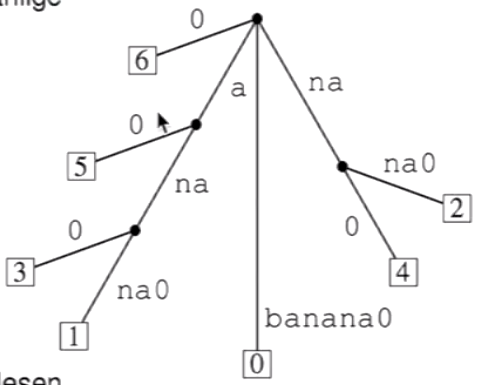
\includegraphics[width=.8\textwidth]{suffixTree}
    \caption{Beispiel für den Suffix-Baum des Strings ``\emph{banana}''}
  \end{figure}
\end{minipage} \\

``Naiv'' ist die Erstellung des Suffixbaums in \( O(n^2) \). Man kann ihn aber auch aus Suffix-Array und LCP-Array in Linearzeit konstruieren. Dazu hängt man die Suffixe sukzessive in der Tiefe ein, die ihr LCP-Wert angibt:

\begin{figure}[H]
  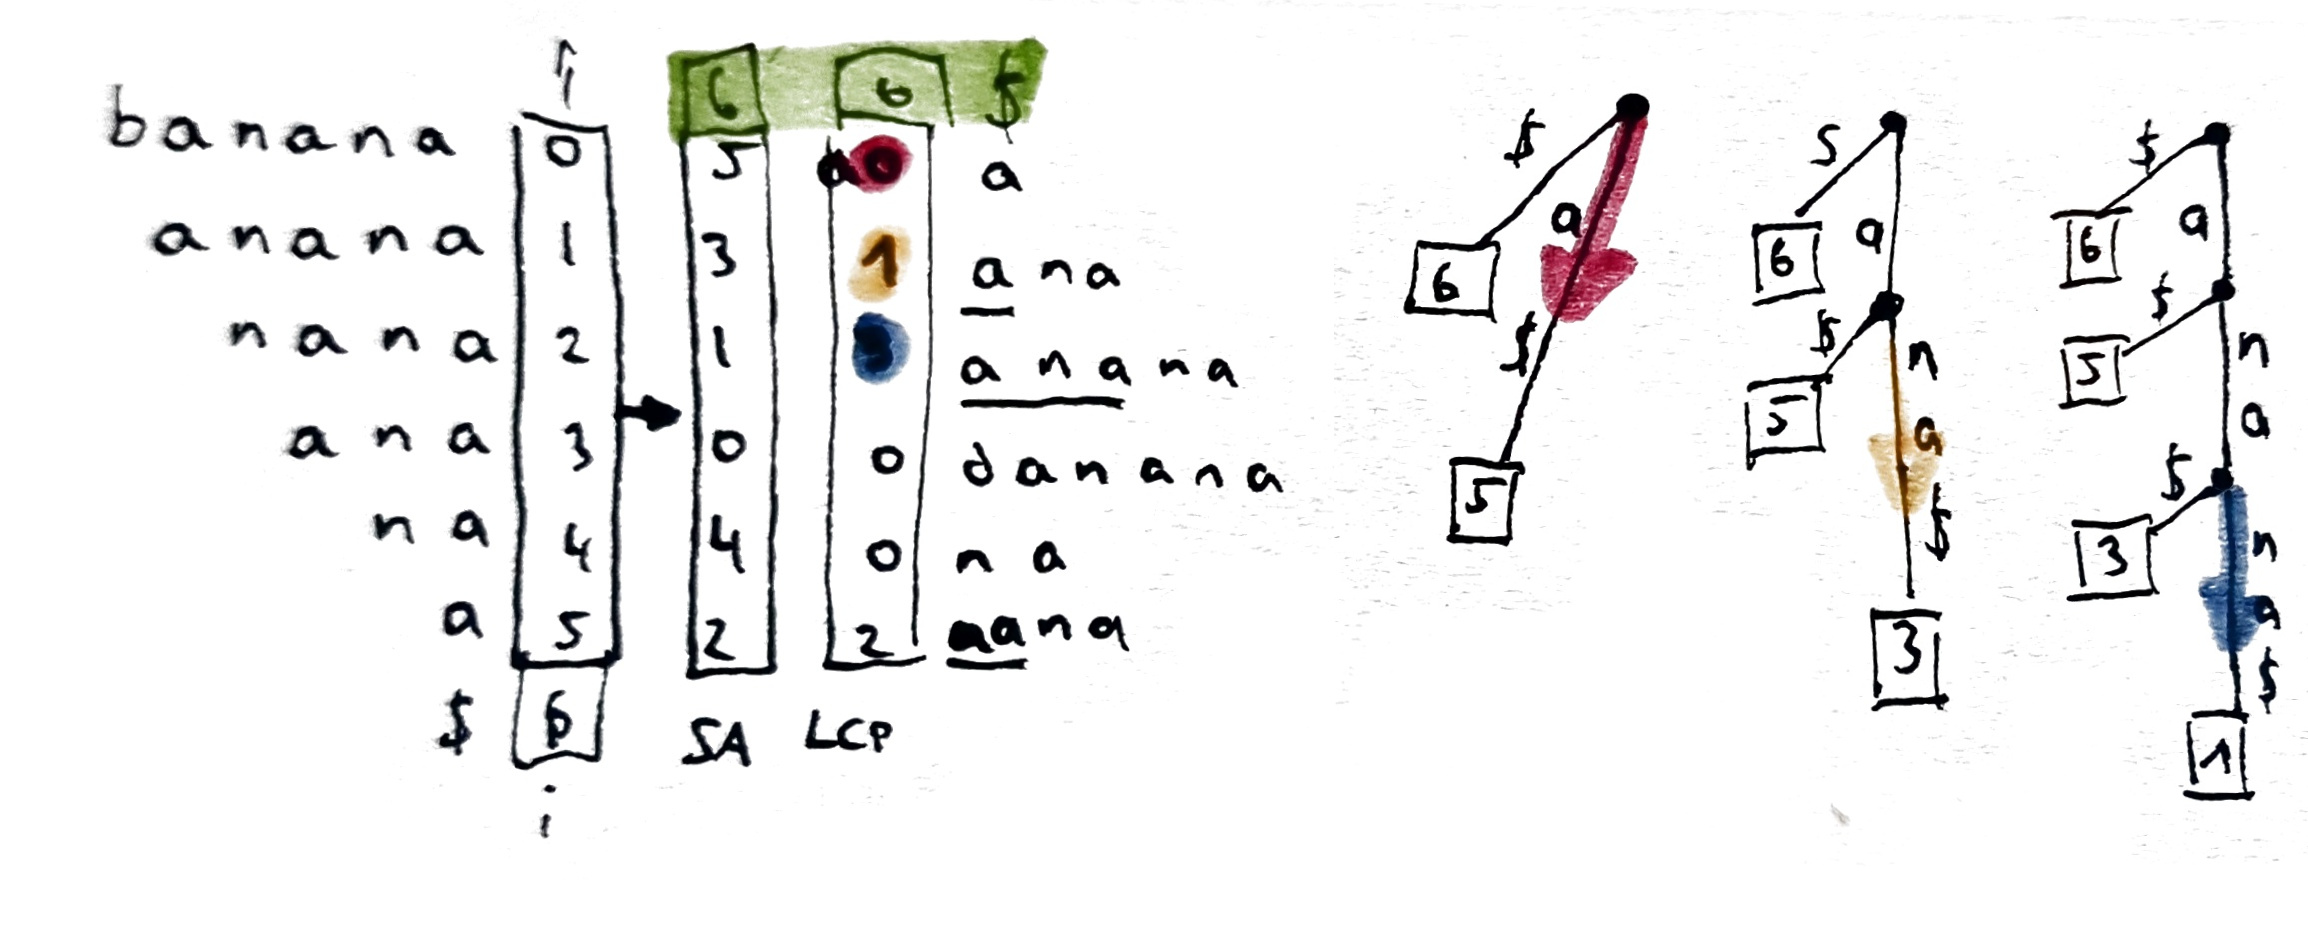
\includegraphics[width=.8\textwidth]{buildSuffixTree}
  \captionsetup{width=.8\textwidth}
  \caption{Sukzessive Konstruktion des Suffix-Baums aus Suffix- und LCP-Array. Zuerst hängt man \$ und das erste Suffix (dessen LCP-Wert immer \( 0 \) ist) an die Wurzel. Anschließend nutzt man den LCP-Wert des darauffolgenden Suffixes (hier \( 1 \)), um festzulegen, wo der Suffix zum Baum hinzugefügt werden muss (durch Pfeile gekennzeichnet)}
\end{figure}

Die Suche in einem Suffix-Baum ist relativ simpel --- man muss lediglich den entsprechenden Kanten entlanglaufen, alle Vorkommen des Patterns liegen im entsprechenden Teilbaum.

Zur Angabe der Komplexitäten sind zwei Fälle zu unterscheiden:

\begin{enumerate}
  \item Die ausgehenden Kanten sind als Arrays der Größe \( \left\vert \Sigma \right\vert \) gespeichert. Dann ist die Suchzeit in \textcolor{green!60!black}{\( O(m) \)} und der Gesamtplatzbedarf in \textcolor{red!80!black}{\( O(n\left\vert \Sigma \right\vert) \)}.
  \item Die ausgehenden Kanten sind als Arrays gespeichert, deren Größe proportional zur Anzahl der Kinderknoten ist. Dann ist die Suchzeit in \textcolor{red!80!black}{\( O(m\log \left\vert \Sigma \right\vert ) \)} und der Gesamtplatzbedarf in \textcolor{green!60!black}{\( O(n) \)}.
\end{enumerate}

\section{Datenkompression}

Eine Anwendung der Suffix-Arrays und -Trees ist die \term{Datenkompression}\index{Kompression}. Inhalt dieser Vorlesung wird ausschließlich die \emph{verlustfreie Textkompression} sein.

\subsection{Wörterbuchbasierte Textkompression}

Für besonders große Datenbestände bietet sich eine \term{wörterbuchbasierte Textkompression}\index{Kompression!wörterbuchbasiert} an. Grundidee ist, \( \Sigma' \subseteq \Sigma^\ast \) zu wählen und \( S \in \Sigma^* \) durch  \( S' = \left\langle s_1', \dots, s_k' \right\rangle \in \Sigma'^\ast \)  zu ersetzen, sodass \( S = s_1' \cdot \cdots \cdot s_k' \) ist. Problem ist der hohe zusätzliche Platzbedarf für das Wörterbuch.

\subsection{Lempel-Ziv-Kompression}

Die \term{Lempel-Ziv-Kompression}\index{Kompression!Lempel-Ziv} baut das Wörterbuch \emph{on the fly} bei Codierung \underline{und} Decodierung, sodass dieses nicht explizit gespeichert werden muss. \\

\begin{figure}[H]
  \begin{minipage}{.42\textwidth}
    \begin{pseudocode}
      \textbf{\textsc{naiveLZCompress}}\( (\left\langle s_1,\dots,s_n \right\rangle, \Sigma) \) \\
      \( D \coloneqq \Sigma \) \quad // init dictionary \\
      \( p \coloneqq s_1 \) \quad // current string \\
      \textbf{for} \( i \coloneqq 2 \) \textbf{to} \( n \) \textbf{do} \\
      \phantom{\enskip} \textbf{if} \( p \cdot s_i \in D \) \textbf{then} \( p \coloneqq p \cdot s_i \) \\
      \phantom{\enskip} \textbf{else} \\
      \phantom{\enskip} \phantom{\enskip} output code for \( p \) \\
      \phantom{\enskip} \phantom{\enskip} \( D \coloneqq D \cup p \cdot s_i \) \\
      \phantom{\enskip} \phantom{\enskip} \( p \coloneqq s_i \) \\
      output code for \( p \)
    \end{pseudocode}
  \end{minipage}
  \begin{minipage}{.55\textwidth}
    \begin{pseudocode}
      \textbf{\textsc{naiveLZDecode}}\( (\left\langle c_1,\dots,c_k \right\rangle) \) \\
      \( D \coloneqq \Sigma \) \\
      output decode\( (c_1) \) \\
      \textbf{for} \( i \coloneqq 2 \) \textbf{to} \( k \) \textbf{do} \\
      \phantom{\enskip} \textbf{if} \( c_i \in D \) \textbf{then} \\
      \phantom{\enskip} \phantom{\enskip} \( D \coloneqq D \cup \text{decode}(c_{i-1}) \cdot \text{decode}(c_i)[1] \)
      \phantom{\enskip} \textbf{else} \\
      \phantom{\enskip} \phantom{\enskip} \( D \coloneqq D \cup \text{decode}(c_{i-1}) \cdot \text{decode}(c_{i-1})[1] \) \\
      \phantom{\enskip} output decode\( (c_i) \) \\
      \ 
    \end{pseudocode}
  \end{minipage}
  \caption{Kompressions- und Dekodierungs-Algorithmus für die Lempel-Ziv-Kompression}
\end{figure}

\begin{figure}[H]
  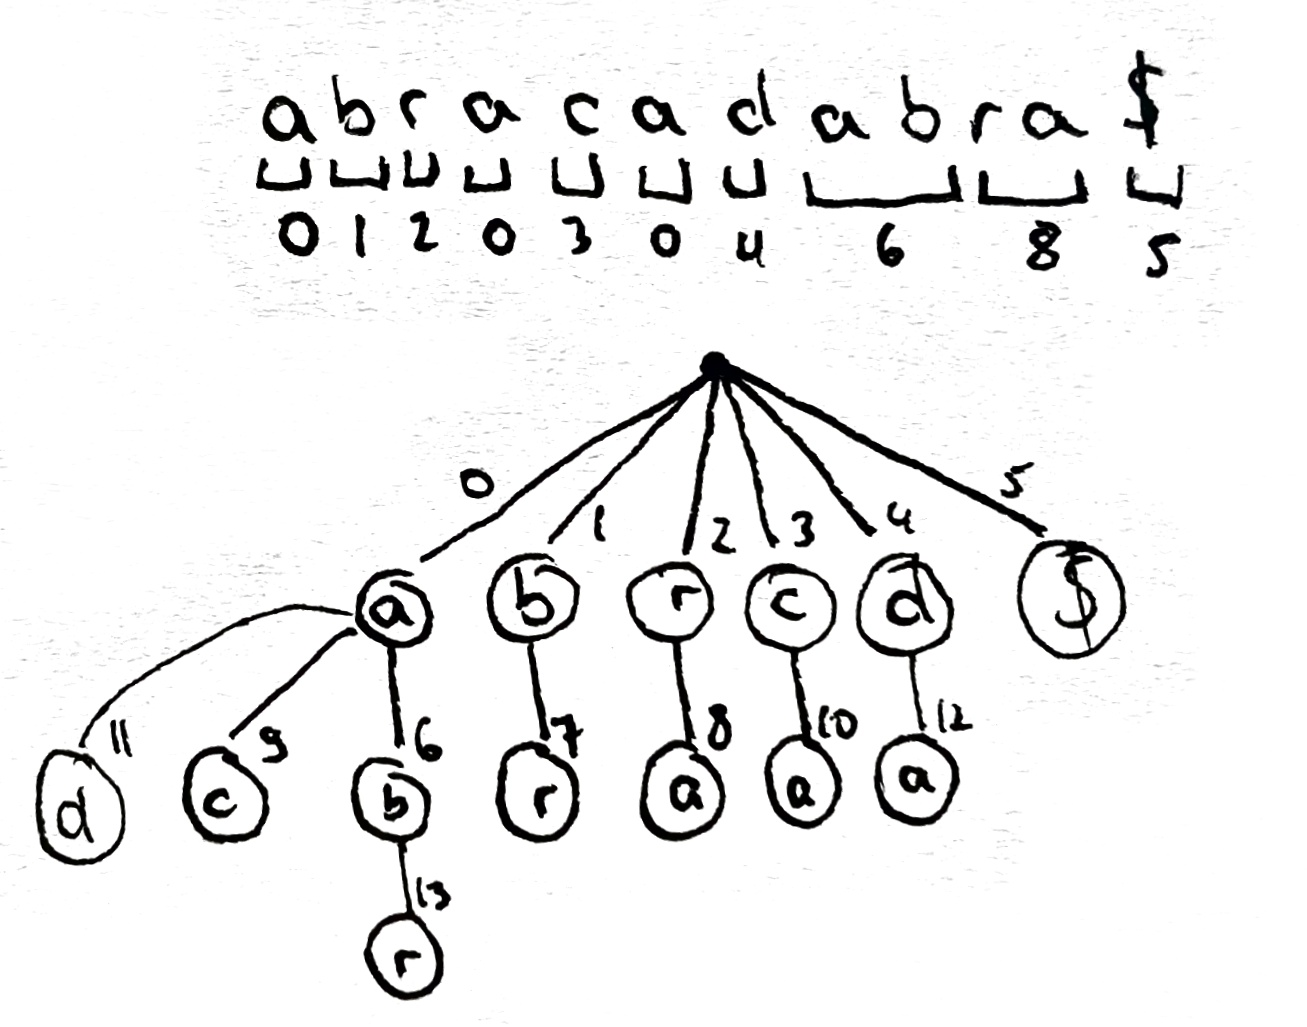
\includegraphics[width=0.4\textwidth]{LZCompress}
  \captionsetup{width=.6\textwidth}
  \caption{Beispiel für das Bilden der Lempel-Ziv-Kompression des Wortes ``\emph{abracadabra}''. Der Baum wird \emph{on the fly} berechnet und nicht übergeben, sondern nur die komprimierte Information und das Alphabet}
\end{figure}